\documentclass{aa}
\usepackage{graphicx}
\usepackage[varg]{txfonts}
\usepackage[%draft, 
colorlinks,citecolor=blue,linkcolor=blue,urlcolor=blue]{hyperref}
\usepackage{amsmath}
\usepackage[usenames]{xcolor}
\usepackage{comment}
\usepackage{multirow}
\usepackage{chngpage}
\usepackage{lscape}
\usepackage{url}
\newcommand{\todo}[1]{{\large $\blacksquare$~\textbf{\color{red}[#1]}}~$\blacksquare$}
\newcommand{\udef}{\stackrel{\mathrm{def}}{=}}
% for tree diagram
\usepackage{forest}
\usepackage{tikz-qtree}
\usetikzlibrary{shadows,trees}

%Selma's comments
\definecolor{Wildstrawberry}{rgb}{1.0, 0.26, 0.64}
\newcommand{\SdM}[1]{{\color{Wildstrawberry}\bf{#1}}}
\newcommand{\newtext}[1]{{\color{ForestGreen}\bf{#1}}}

\renewcommand{\labelitemii}{$\bullet$}
\newcommand{\kms}{{\,\mathrm{km\ s^{-1}}}}
\newcommand{\Msun}{{\mathrm{M}_\odot}}

\DeclareRobustCommand{\Eqref}[1]{Eq.~\ref{#1}}
\DeclareRobustCommand{\Figref}[1]{Fig.~\ref{#1}}
\DeclareRobustCommand{\Tabref}[1]{Table~\ref{#1}}
\DeclareRobustCommand{\Secref}[1]{Sec.~\ref{#1}}

% \defcitealias{tauris:98}{TT98}
% \defcitealias{ramirez-agudelo:15}{R-A15}

\interfootnotelinepenalty=10000    % brute-forces the footnote not to break over two pages

  
\begin{document}

\title{VFTS682: a confirmed dynamical ejection?}

\author{M.~Renzo\inst{1} \and \todo{TBD}% S.~E.~de~Mink\inst{1} \and
  % S.~Justham\inst{2,3} \and A.~de~Koter\inst{1} \todo{etc..order to be decided}
  .} 

\institute{{Astronomical Institute Anton Pannekoek, University of
    Amsterdam, 1098 XH Amsterdam, The Netherlands}
  % \and{School of Astronomy \& Space Science, University of the Chinese
  %   Academy of Sciences, Beijing 100012, China}
  % \and{National Astronomical Observatories, Chinese Academy of
  %   Sciences, Beijing 100012, China}
}
  
\offprints{M.~Renzo, \href{mailto:m.renzo@uva.nl}{m.renzo@uva.nl}}
\date{}
\abstract{}

\keywords{stars: kinematics, stars: runaways, stars: individual: VFTS682}
\maketitle{}

\section{Introduction}
\label{sec:intro}

How do stars form is one longstanding question in astrophysics
\cite{lada:03, zinnecker:07}. It is particularly difficult for massive stars, because these are intrinsically rare
\citep[e.g.,][]{salpeter:55,kroupa:01, schneider:18}, evolve fast, and
remain enshrouded in their parent cloud during the formation
process. Moreover, observations of young massive stars reveal a
complicated multipliticy structure which requires
explanation \citep[][]{kobulnicky:07,mason:09,sana:11,sana:12,kiminki:12,chini:12,kobulnicky:14,almeida:17,demarco:17}. Understanding massive star formation, possibly as a
function of metallicity, is a key question given the present and upcoming
transient survey \citep[e.g., LSST, BlackGem, LIGO/Virgo O3][]{}\todo{ref} which
will reveal transients associated to massive stars
evolution and death.

The second data release (DR2) from the Gaia satellite
\cite[][]{gaia:16,brown:18} allows us to test
these hypothesis using one particular star, VFTS682. 
This star is a
very massive \citep[$M_\mathrm{ZAMS}\simeq150\,M_\odot$,][]{bestenlehner:11,schneider:18} WNh5 star in the 30 Doradus region
of the Large Magellanic Cloud (LMC), and it is presently observed at a
projected distance of $\sim$$29$\,pc from the nearest cluster of
massive stars R136 \citep[][]{bestenlehner:11}. Based on the extremely high mass of this star and
its present day apparent isolation, \cite{bestenlehner:11} proposed it
might be a candidate for isolated star formation, or a ``slow runaway'' ejected
from R136 in the past. This second option is also supported by the
N-body simulations of \cite{fujii:11, banerjee:12}.   Many other
very massive stars are present in the surroundings of R136, and a more
detailed analysis on the larger sample is desirable.


Massive stars can in principle be ejected from R136 as a consequence of dynamical
interactions \citep[][]{poveda:67,leonard:91, evans:10, fujii:11,
  allison:12, oh:16}, or by the disruption of a binary by the first
core-collapse supernova
\citep[][]{zwicky:57,blaauw:61,dedonder:97,eldridge:11,renzo:18}. However,
R136 has an estimated age of $\lesssim2$\,Myr \citep[][]{sabbi:12}, which is
shorter than the shortest stellar lifetime
\citep[$\sim$3\,Myr, e.g.,][]{zapartas:17}, so one would not expect the binary
disruption scenario to be relevant for this cluster.


In this study, we combine the radial velocity measurements from the
VFTS survey \citep[][]{evans:11} with the proper motion from Gaia DR2
to reconstruct the three-dimensional velocity of VFTS682, and test the
hypothesis that this star was ejected from R136. We discuss in
\Secref{sec:sample} the data for VFTS682, and the selection of stars
used to define a local reference frame. Our results
indicate that R136 is a bona fide runaway star (\Secref{sec:runaway}), therefore isolated star formation is \emph{not}
required to explain it. We also find that a dynamical ejection from
R136 is compatible with the direction of its velocity
vector. \todo{double check the following}
However, we find a mild discrepancy between the apparent age of
VFTS682, its kinematic age, and the age estimates for R136 (\Secref{sec:r136_origin}).  We conclude
with a very brief discussion on the implications for theories of
star formation, N-body interactions, and binary evolution in
\Secref{sec:discussion}.

\section{Gaia DR2 data selection}
\label{sec:sample}

VFTS682 is labeled in the Gaia DR2
catalog\footnote{\url{https://vizier.u-strasbg.fr/viz-bin/VizieR-3?-source=I/345/gaia2}} with the
source id 4657685637907503744. The star has a
\texttt{visibility\_period} = 17, which counts how many observations have
been used to reconstruct its astrometric solution
\citep[][]{lindengren:18}. Its reported G-band
magnitude is 15.65, cf. the V-band magnitude of 16.08
\citep[][]{evans:11, bestenlehner:11}, and the reported
\texttt{astrometric\_excess\_noise} = 0. These values suggest that the Gaia
data for VFTS682 are trustworthy. However, the effective temperature
reported in Gaia DR2 is one order of magnitude lower than what found by
\cite{bestenlehner:11}, and the best fit parallax of this star is
negative. We do not use the effective temperature of the star anywhere
in this study, and we attribute the unphysical value of the parallax
to the large distance to the LMC. Our main findings do not rely on the
parallax nor the effective temperature values reported in the Gaia DR2
catalog.

%% should I really mention the line of sight velocity? Not really
%% using it...

We retrieve for VFTS682 the position in right ascension (RA) and declination (DE)
in the IGCS frame \cite[][]{brown:18}, its
proper motion components ($\mu_\mathrm{RA}$, and $\mu_\mathrm{DE}$,
respectively). For the radial velocity of VFTS682 and of the 30 Doradus
region as a whole, we instead use the VFTS data
as quoted in \cite{bestenlehner:11}. \Tabref{tab:vfts682} lists the values adopted throughout
this work for each of these quantities.

\begin{table}[tbp]
  \centering
    \caption{Astrometric parameters for VFTS682. The peculiar radial
    velocity $\delta v_\mathrm{rad}$ is obtained as the difference
    between the average radial velocity of the 30 Doradus region
    ($270\pm10\kms$) minus the radial velocity measured from the HeII $\lambda4686$
    line for VFTS682 ($315\pm15\kms$).}

  \begin{tabular}[htbp]{l|c|c}
    Parameter & Value & Source\\ \hline\hline
    RA \hfill[degree] &  \phantom{-}84.73 $\pm$  0.03 & \multirow{4}{*}{Gaia DR2}\\
    DE \hfill [degree] & -69.07 $\pm$  0.05  & \\
    $\mu_\mathrm{RA}$  \hfill[$\mathrm{mas\ yr^{-1}}$] & \phantom{-0}1.84 $\pm$ 0.07 & \\
    $\mu_\mathrm{DE}$  \hfill[$\mathrm{mas\ yr^{-1}}$] & \phantom{-0}0.78 $\pm$ 0.08& \\
    $\delta v_\mathrm{rad}$  \hfill[$\kms$] & \phantom{0}-45 $\pm$ 25 & \cite{bestenlehner:11}\\
    \hline
  \end{tabular}
  \label{tab:vfts682}
\end{table}

To compare the astrometry of VFTS682 and derive its peculiar motion,
we then select data from the Gaia DR2 catalog for two regions: the
``surroundings'' of VFTS 682, and the ``R136 cluster''. The
surrounding region is defined by all the stars in a target of 10 arcminutes around
VFTS682 fulfilling the following criteria: we require \texttt{visibility\_period} $\geq$ 5,
\texttt{astrometric\_excess\_noise} < 1, the error on the proper
motion components to be smaller than 0.1\,$\mathrm{mas\ yr^{-1}}$,
and the proper motion components themselves to be smaller than
2\,$\mathrm{mas\ yr^{-1}}$ in absolute value. At the distance to the
LMC, $1\mathrm{mas\ yr^{-1}}\simeq250\,\kms$ \citep[e.g.,][]{lennon:18}, so the cut on the values
of the proper motions removes stars that would have projected
tangential velocities in excess of $\sim$500\,$\kms$, which are most
likely to be foreground stars. We checked that the additional
requirement of having parallaxes smaller than $1\,\mathrm{mas\
  yr^{-1}}$ does not reduces further our sample. This selection yields 437 stars.

The ``R136 cluster'' is effectively defined by taking all the stars
in a region of 50 arcseconds around R136a, one of the most massive members of
the cluster itself \citep[][]{crowther:10}, requiring the same
``quality'' criteria applied above. This selection yields 42 stars.
\todo{improve definition of stars from R136, describe accordingly -- check with Danny}

Throughout this study, we assume the same distance of $50$\,kpc to the star, and to
the 30 Doradus region as a whole.% , since the parallax for VFTS682
% listed in the Gaia DR2 catalog is negative. %% this is what makes the
%                                 % LOS velocity useless...how to improve?

For each of the two local rest frames (``surroundings'' and ``R136
cluster''), we compute the average transverse velocity as:

\begin{equation}
  \label{eq:mean}
  \langle \mu_i\rangle = \frac{\sum_\mathrm{stars}\frac{1}{\Delta
      \mu_i}\mu_i}{\sum_\mathrm{stars} \frac{1}{\Delta \mu_i}} \ \ , \
  \ \Delta \langle \mu_i\rangle = \frac{\sqrt{N}}{\sum_\mathrm{stars}
    \frac{1}{\Delta \mu_i}} \ \ ,
\end{equation}
where $i = \mathrm{RA}, \mathrm{DEC}$, and $\Delta \mu_i$ is the error
on the proper motion component reported by Gaia, and the sums run over
all the $N$ stars of the frame considered. We evaluate each proper motion
component separately. 

The data retrieved, and the ipython notebook used for the analysis
presented here will be made available at \todo{probably git repo on bitbucket?}. 

\section{The kinematics of VFTS682}
\label{sec:results}

\subsection{Is it a runaway star?}
\label{sec:runaway}
We first address the question of whether VFTS682 is a typical star
from the kinematic point of view, or whether it is a runaway star with
a significantly large peculiar velocity compared to its surrounding population. The former is what should
be expected if it formed where we observe it today, in relative
isolation from other massive stars.

Using the 437 stars selected as the ``surrounding population'' in
\Secref{sec:sample} and shown in blue in \Figref{fig:main}, we find averaged proper motion components of
$\langle\mu_\mathrm{RA}^\mathrm{sur}\rangle = 1.695\pm0.003\,\mathrm{mas\ yr^{-1}}$ and
$\langle\mu_\mathrm{DE}^\mathrm{sur}\rangle = 0.691\pm0.003\,\mathrm{mas\ yr^{-1}}$. Subtracting these values from the
proper motions of VFTS682 (see \Tabref{tab:vfts682}), we obtain the
components of proper motion of the star relative to the surrounding region
$\mu^\mathrm{sur}_\mathrm{RA} = 0.15\pm 0.07\,\mathrm{mas\ yr^{-1}}$ and $\mu^\mathrm{sur}_\mathrm{DE} =
0.09\pm 0.08\,\mathrm{mas\ yr^{-1}}$. %% note that the error budget is
% dominated by VFTS682
These can be converted in the
the components of the transverse velocity $v^\mathrm{sur}_\mathrm{RA}=35\pm17\,\kms$,
$v^\mathrm{sur}_\mathrm{DE}=22\pm19\,\kms$, assuming a distance of
50\,kpc (we do not account for the uncertainty in the distance
estimate when propagating errors). The radial velocity from
\cite{bestenlehner:11} then gives the third component along
the line of sight, allowing us to calculate the speed of the star:

\begin{equation}
  \label{eq:speed_around}
  v^\mathrm{sur} = \sqrt{\left(v^\mathrm{sur}_\mathrm{RA}\right)^2
    +\left(v^\mathrm{sur}_\mathrm{DE}\right)^2+\left(\delta v_\mathrm{rad}\right)^2} = 61 \pm 22
  \, \kms \ .
\end{equation}
This value for the three-dimensional speed of VFTS682 with respect the
surrounding stars make it a ``bona fide'' runaway star.

\subsection{Does it come from the R136 cluster?}
\label{sec:r136_origin}

The inset plot in \Figref{fig:main} shows a zoom in of the region
around R136 which includes VFTS682. Stars belonging to our ``R136
cluster'' group are shown in green (see \Secref{sec:sample}), together with their proper motion
as listed in the Gaia DR2 catalog.
To test the hypothesis that VFTS682 was indeed ejected from this region, we check the
orientation of its proper motion relative to these stars. We further
consider also the kinematic age of the star.

We begin by evaluating the average proper motion for the stars
representing the cluster. This is necessary to constrain the actual velocity
obtained by VFTS682 at its ejection. By using \Eqref{eq:mean} we find  
$\langle\mu_\mathrm{RA}^{R136}\rangle = 1.750\pm0.008\,\mathrm{mas\ yr^{-1}}$
and $\langle\mu_\mathrm{DE}^\mathrm{R136}\rangle =
0.742\pm0.009\,\mathrm{mas\ yr^{-1}}$. Therefore, using the values
from \Tabref{tab:vfts682}, we obtain the components of the proper
motion for VFTS682 relative to R136 $\mu^{R136}_\mathrm{RA} = 0.09\pm 0.07\,\mathrm{mas\ yr^{-1}}$ and $\mu^{R136}_\mathrm{DE} =
0.04\pm 0.08\,\mathrm{mas\ yr^{-1}}$.\todo{improve numbers by
  selecting better sample}.
\todo{discuss if direction is compatible
The error cone, obtained by
propagating the errors on the proper motion components indicates that
R136 is indeed the most likely origin, as expected by \cite{fujii:11,
  banerjee:12}.
}

Assuming again a distance of 50\,kpc and
not considering the error on the distance, we can convert these into
the components of the tangential velocity relative to R136,
$v^\mathrm{R136}_\mathrm{RA}=21 \pm 18\, \kms$ and $v^\mathrm{R136}_\mathrm{DE}=10
\pm 21\,\kms$. Finally, using the peculiar line of sight velocity
from \cite{bestenlehner:11}, we obtain the three-dimensional peculiar
velocity of VFTS682 with respect to R136

\begin{equation}
  \label{eq:speed_R136}
  v^\mathrm{sur} = \sqrt{\left(v^{R136}_\mathrm{RA}\right)^2
    +\left(v^{R136}_\mathrm{DE}\right)^2+\left(\delta v_\mathrm{rad}\right)^2} = 51 \pm 23
  \, \kms \ .
\end{equation}



\todo{kinematic age}


\begin{figure*}[htbp]
  \centering
  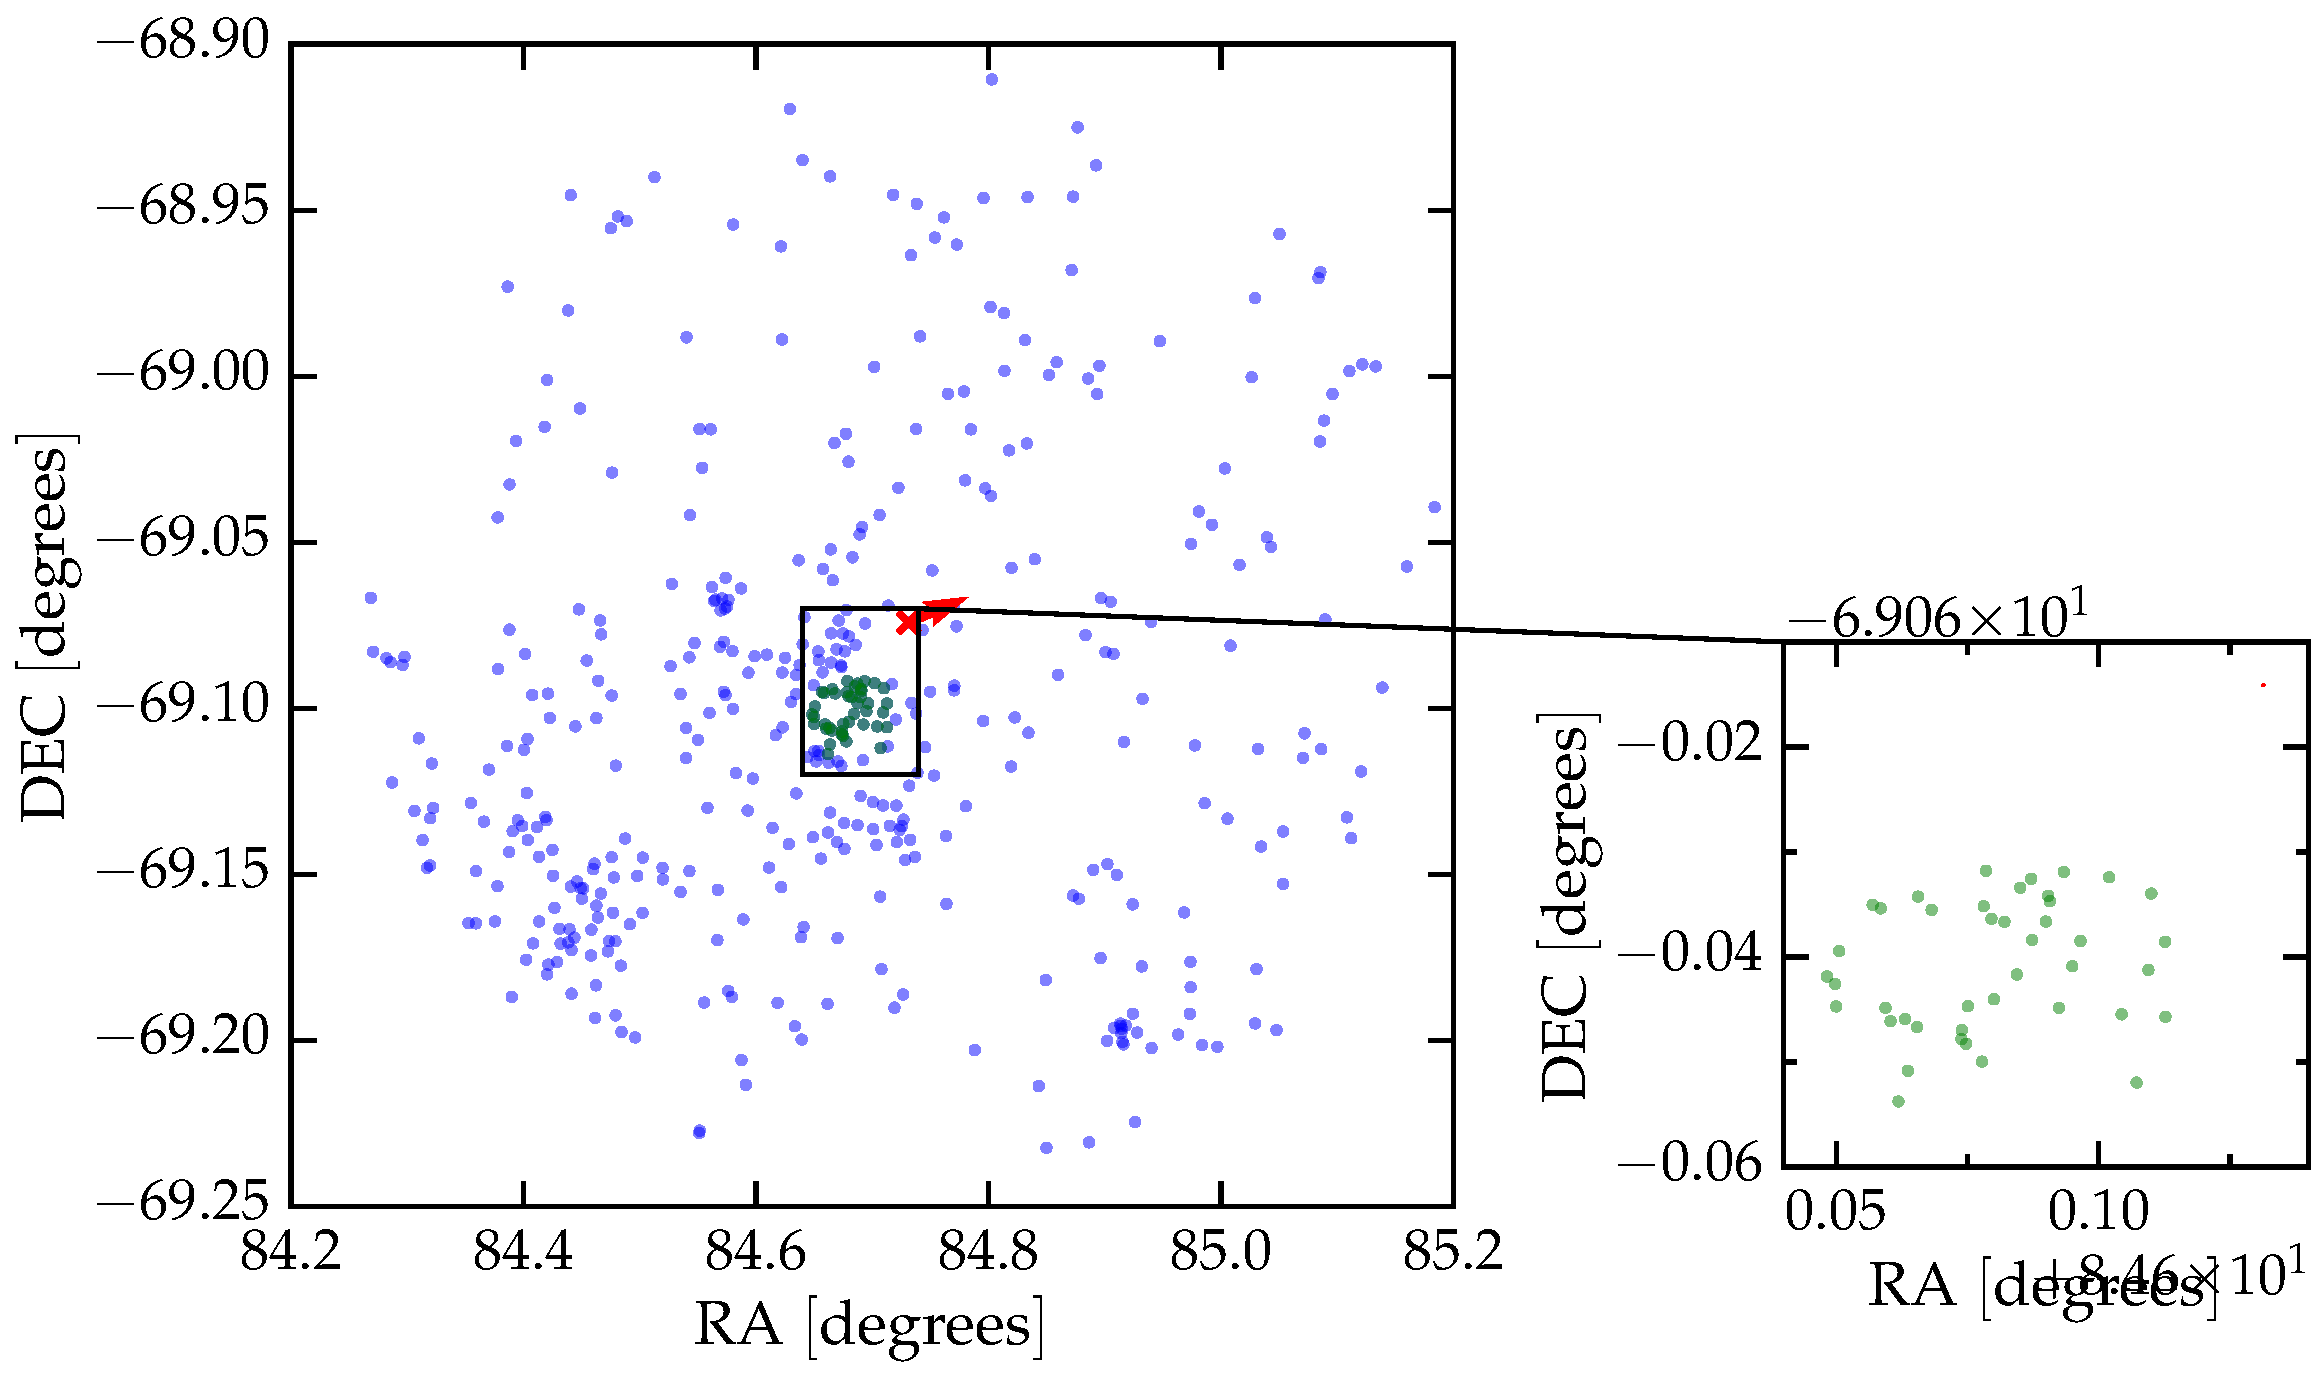
\includegraphics[width=\textwidth]{./figures/main_plot}  
  \caption{position and projected relative velocity to
    R136. \todo{orient properly, load  picture on background, add cone
      of uncertainty, maybe show pm for all stars in inset?}}
  \label{fig:main}
\end{figure*}

\section{Summary and Discussion}
\label{sec:discussion}

\begin{itemize}
\item VFTS682 is a bona fide runaway with $v\sim60\,\mathrm{km\
    s^{-1}}$ thrown out from R136. Both its speed and the age of the
  cluster are consitent with a dynamical ejection.
  \item VFTS682 comes from R136 as was expected by
  \cite{bestenlehner:11, fujii:11, banerjee:12}, so it does not
  require isolated SFH to be explained
\item apparent age tension (connect to VFTS16 as well).
\item is R136 a single young cluster or a merger
\item estimate the influence of the gravitational potential of R136,
  what is its total mass and relaxation time?
\end{itemize}

Random notes: $v\sin(i)<200\,\mathrm{km\ s^{-1}}$ form \cite{schneider:18}, age $1.0\pm 0.2$\,Myr
from \cite{schneider:18}

\bibliographystyle{aa}
\bibliography{bibliography/vfts682}

\begin{acknowledgements}
  The background image of \Figref{fig:main} is based on observations made with ESO Telescopes at the La Silla Observatory under programme ID 076.C-0888, processed and released by the ESO VOS/ADP group.
  We are grateful to S.~Torres for extremely useful discussions on the
  Gaia DR2 dataset.
\end{acknowledgements}
\end{document}




%%% Local Variables:
%%% mode: latex
%%% TeX-master: t
%%% End:
